\section{Introduction}
\label{introduction:section}

Classical computing has advanced considerably over the decades and now forms the backbone of modern technological infrastructure. %
In contrast, quantum computing introduces a fundamentally new paradigm for information processing, grounded in the principles of quantum mechanics. This paradigm enables the solution of computational problems that are beyond the practical capabilities of classical methods. %

The core distinction between classical and quantum computing lies in the way information is represented and manipulated. %
Classical computers operate on bits that exist in one of two binary states—$0$ or $1$. In contrast, quantum computers use quantum bits, or \emph{qubits}, which exhibit the quantum phenomena of \emph{superposition} and \emph{entanglement}. %
Superposition enables a qubit to exist in multiple states at once, thereby allowing parallel evaluation of many possibilities. Entanglement creates correlations between qubits such that the state of one qubit can instantaneously influence the state of another, regardless of the distance between them. %
These phenomena enable quantum systems to represent and manipulate exponentially many states simultaneously,
and to encode complex correlations that classical systems cannot efficiently reproduce, resulting in powerful computational advantages. %

\begin{figure}
\center
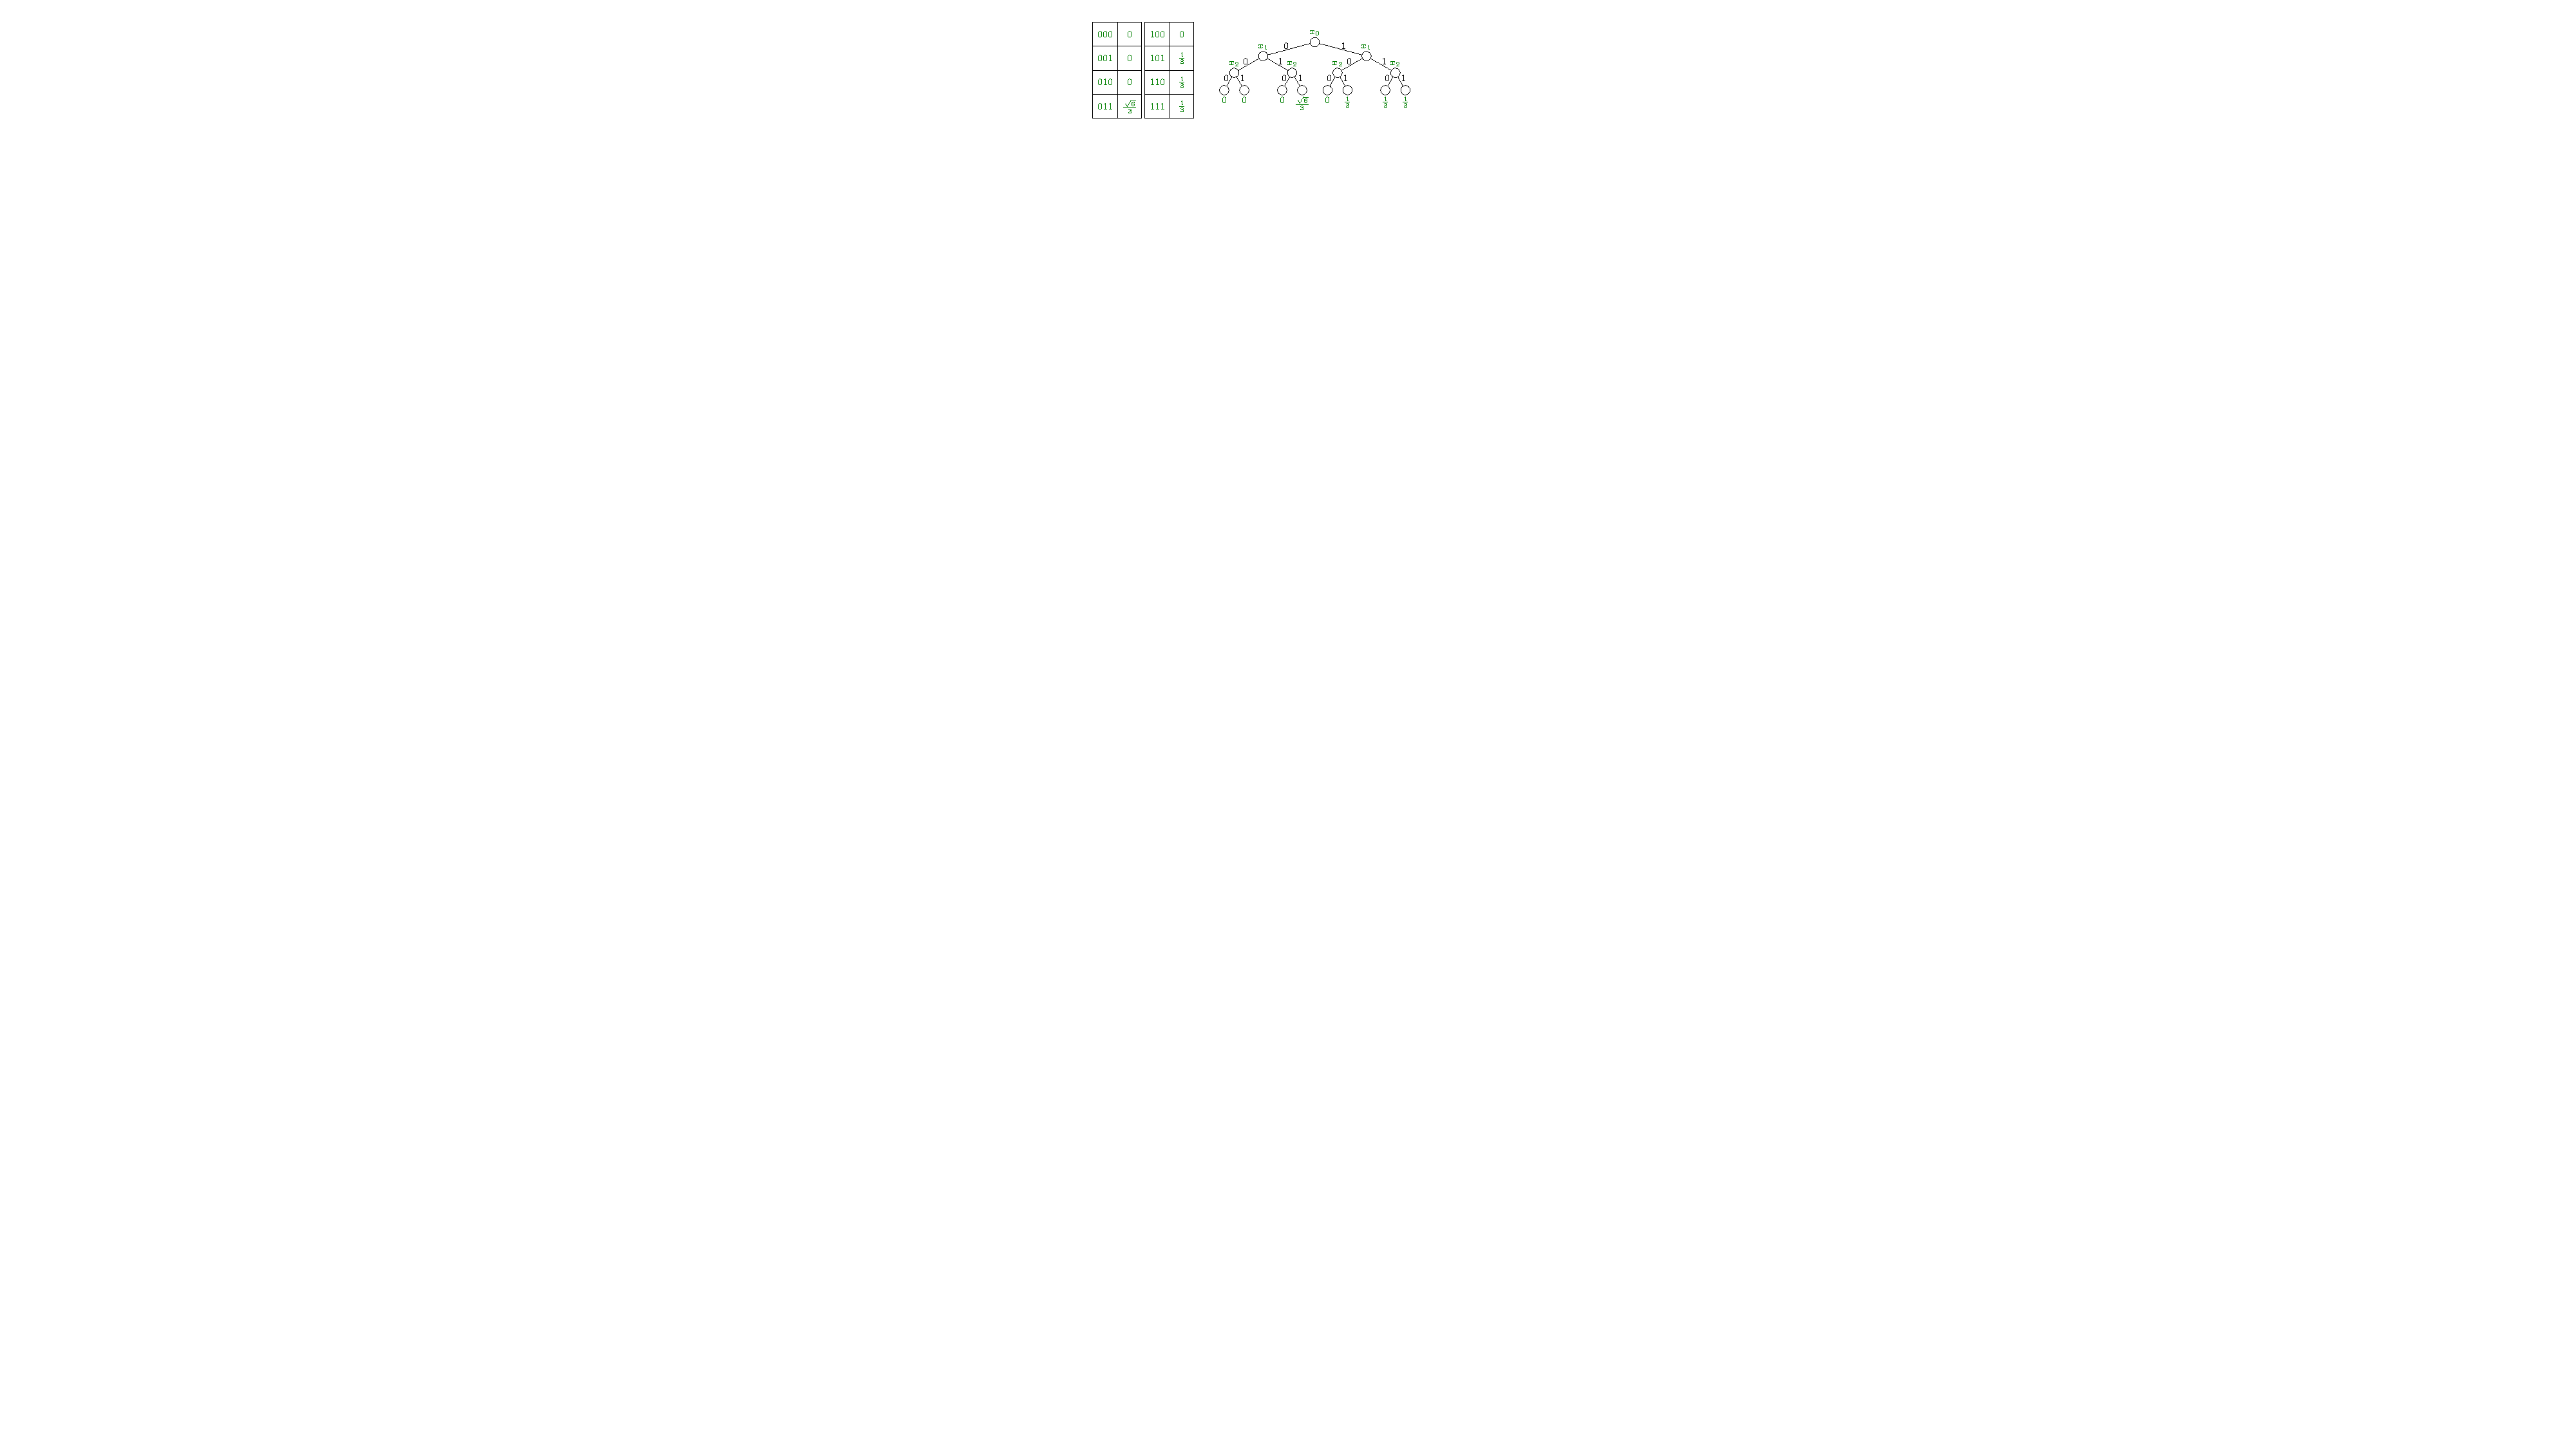
\includegraphics[scale=0.95]{Figures/Trees/Tree}
\caption{A quantum state with three qubits and its tree representation.
The system can be in any of the eight states, with the probability given in the table.}
\label{qustate:tree:fig}
\end{figure}

\cref{qustate:tree:fig} depicts a quantum state consisting of three qubits.\footnote{Throughout the text, we illustrate the challenges encountered in verifying quantum circuits through examples. %
For clarity, these examples are simplified. Full technical details are beyond the scope of this document and can be found, for example, in~\citep{10.5555/1408782}.} In a classical circuit, the system would occupy a single \emph{basis} state from among the eight possible configurations: $000$, $001$, \ldots, $111$. %
By contrast, a quantum system can exist in a superposition of all eight basis states simultaneously, each associated with a specific probability amplitude.

A quantum state can be interpreted as a distribution over basis states, where each state is assigned a complex amplitude. This distribution may be visualized as a tree, in which each path from the root to a leaf corresponds to a basis state, and each leaf stores a complex-valued amplitude. 
%
Unlike classical probabilistic models, quantum amplitudes are complex numbers, and the sum of the squares of their absolute values must equal one.\footnote{An \emph{amplitude} generalizes the classical notion of probability. The square of the absolute value of a complex amplitude gives the corresponding probability. The use of complex numbers permits constructive and destructive interference, allowing for the cancellation of certain outcomes.} 
%

A primary objective in the field of quantum computing is to achieve \emph{quantum supremacy}---the point at which quantum computers can solve problems that are infeasible for even the most powerful classical supercomputers. 
%
Reaching this milestone would result in exponential speedups for specific computational tasks. 
%
%
Although the field is still in an early phase of practical realization, quantum computing applications are growing rapidly. %
In the near term, hybrid systems integrating classical and quantum processors are expected to gain prominence. Looking ahead, quantum supremacy could revolutionize entire industries by solving problems that were previously considered intractable. 
%
Potential application areas for quantum technologies include medical diagnostics, cryptography, secure communications infrastructure, and autonomous systems, among others. 
%
These domains typically require stringent reliability and safety standards, as they cannot tolerate critical system failures. Consequently, they demand rigorous certification procedures and robust assurance mechanisms. Ensuring the reliability of quantum systems is therefore of critical importance. %
%
Nevertheless, verifying quantum systems presents formidable challenges. Their probabilistic behavior, combined with the exponential growth of state spaces as the number of qubits increases, introduces substantial complexity. %

In this paper, we describe initial steps toward tackling these challenges by leveraging insights from our community's extensive experience in verifying classical systems. 
%
Building on this foundation, we will also propose a roadmap for the development of new verification frameworks that transfer the proven strengths of classical approaches—such as concise property specification, accurate fault detection, automation, and scalability—into the quantum domain.

We envision significant added value in bridging two complementary areas of computer science, especially when established techniques from a mature field are adapted to address complex problems in an emerging domain.
%
This work embodies such interdisciplinary integration by applying well-developed methods from logic, automata theory, and symbolic verification to the problem of ensuring the correctness of quantum programs.
%
 
We present a novel application of automata theory—a foundational discipline in formal verification—to the verification of quantum systems.
%
Our methodology integrates automata-based reasoning with symbolic representations tailored for the automated analysis of quantum behavior.
%
The goal is to generalize core concepts from classical verification, such as state-space exploration and symbolic reasoning, into the quantum realm, thereby enabling the adaptation of robust classical paradigms to quantum computing, where formal assurances are essential.
%
Interestingly, this approach also opens new avenues for research in automata theory itself, as the mathematical structures encountered in quantum systems introduce novel challenges and opportunities.
%
It establishes a conceptual bridge between quantum program verification and automata theory, fostering potential for new theoretical developments and extending the expressive and analytical power of automata-based techniques into the context of quantum computation.
%
We will give a high-level description  of how to  develop {\it symbolic representations}, based on {\it automata}, that serve as a theoretical and algorithmic foundation for efficiently modeling the state spaces of quantum circuits. These representations are grounded in the idea of modeling quantum states as binary trees, where each path from the root to a leaf corresponds to a computational basis state (see \cref{qustate:tree:fig}). 

In the remainder of the paper, we first describe the modeling of quantum states, gates, and circuits, followed by a formalization of the verification problem.
Subsequently, we outline a roadmap highlighting potential challenges and opportunities in the verification of quantum systems.
